\documentclass{standalone}
\usepackage{tikz}
\usetikzlibrary{patterns, positioning}


\begin{document}
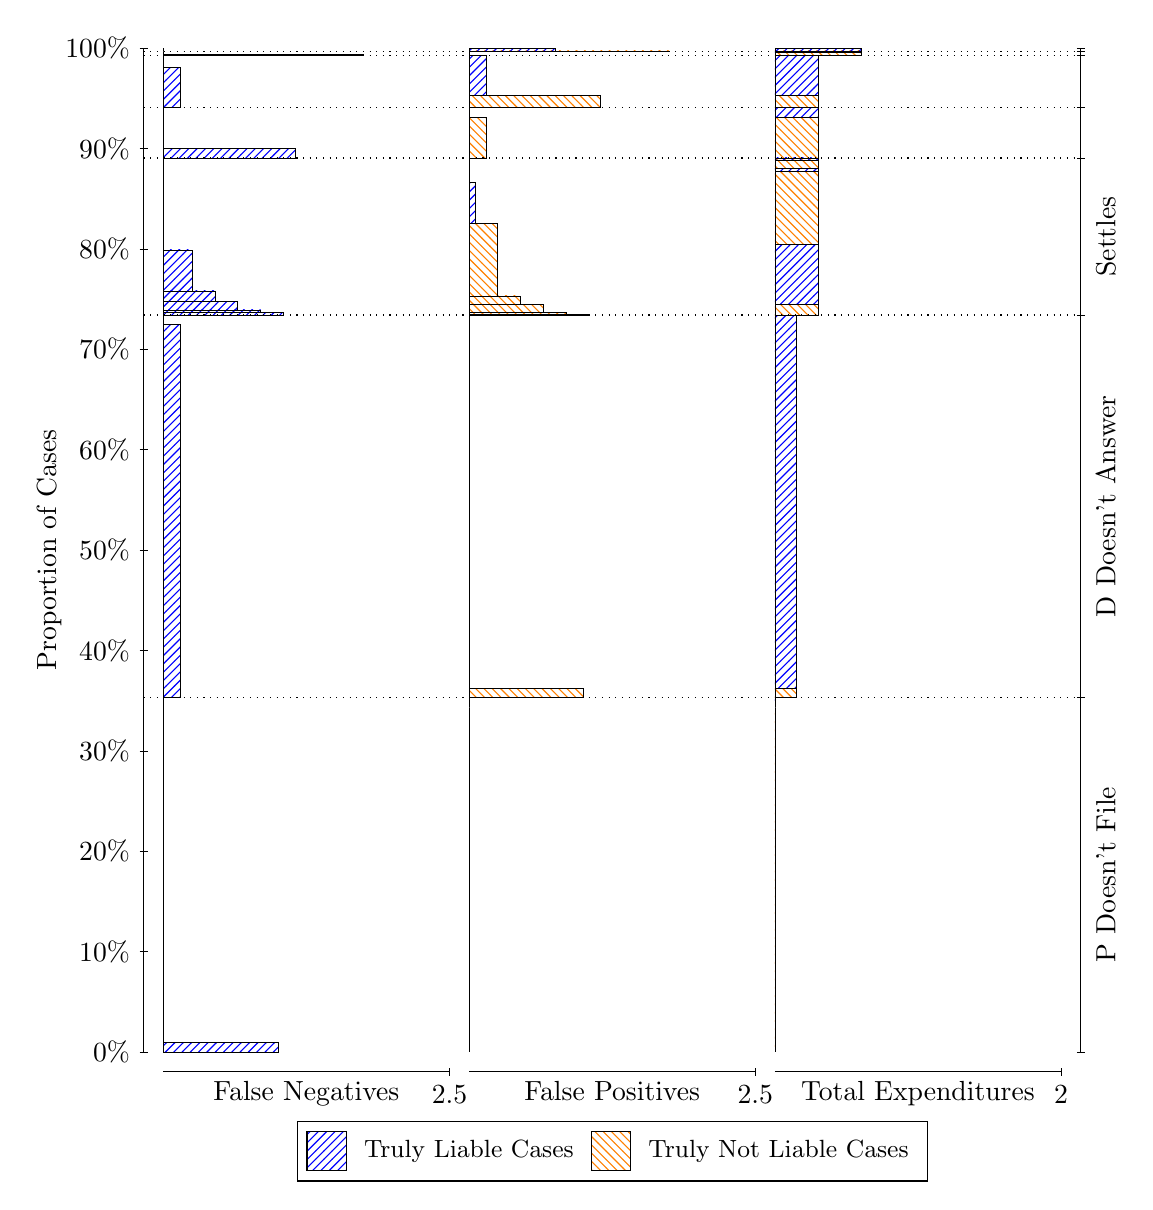
\begin{tikzpicture}
\draw[black, very thin] (1.5,1.75) -- (1.5,14.5);
\node[rotate=90, text=black, anchor=center] at (0.3, 8.125) {Proportion of Cases};
\draw[black, very thin] (1.45,1.75) -- (1.55,1.75);
\node[text=black, anchor=east] at (1.45, 1.75) {0\%};
\draw[black, very thin] (1.45,3.025) -- (1.55,3.025);
\node[text=black, anchor=east] at (1.45, 3.025) {10\%};
\draw[black, very thin] (1.45,4.3) -- (1.55,4.3);
\node[text=black, anchor=east] at (1.45, 4.3) {20\%};
\draw[black, very thin] (1.45,5.575) -- (1.55,5.575);
\node[text=black, anchor=east] at (1.45, 5.575) {30\%};
\draw[black, very thin] (1.45,6.85) -- (1.55,6.85);
\node[text=black, anchor=east] at (1.45, 6.85) {40\%};
\draw[black, very thin] (1.45,8.125) -- (1.55,8.125);
\node[text=black, anchor=east] at (1.45, 8.125) {50\%};
\draw[black, very thin] (1.45,9.4) -- (1.55,9.4);
\node[text=black, anchor=east] at (1.45, 9.4) {60\%};
\draw[black, very thin] (1.45,10.675) -- (1.55,10.675);
\node[text=black, anchor=east] at (1.45, 10.675) {70\%};
\draw[black, very thin] (1.45,11.95) -- (1.55,11.95);
\node[text=black, anchor=east] at (1.45, 11.95) {80\%};
\draw[black, very thin] (1.45,13.225) -- (1.55,13.225);
\node[text=black, anchor=east] at (1.45, 13.225) {90\%};
\draw[black, very thin] (1.45,14.5) -- (1.55,14.5);
\node[text=black, anchor=east] at (1.45, 14.5) {100\%};

\draw[black, very thin] (13.4,1.75) -- (13.4,14.5);
\draw[black, very thin] (13.35,1.75) -- (13.45,1.75);
\node[anchor=west] at (13.35, 1.75) {};
\draw[black, very thin] (13.35,6.2508) -- (13.45,6.2508);
\node[anchor=west] at (13.35, 6.2508) {};
\draw[black, very thin] (13.35,11.109) -- (13.45,11.109);
\node[anchor=west] at (13.35, 11.109) {};
\draw[black, very thin] (13.35,13.104) -- (13.45,13.104);
\node[anchor=west] at (13.35, 13.104) {};
\draw[black, very thin] (13.35,13.742) -- (13.45,13.742);
\node[anchor=west] at (13.35, 13.742) {};
\draw[black, very thin] (13.35,14.408) -- (13.45,14.408);
\node[anchor=west] at (13.35, 14.408) {};
\draw[black, very thin] (13.35,14.455) -- (13.45,14.455);
\node[anchor=west] at (13.35, 14.455) {};
\draw[black, very thin] (13.35,14.5) -- (13.45,14.5);
\node[anchor=west] at (13.35, 14.5) {};

\draw[black, very thin, pattern color=blue, pattern=north east lines] (1.75,1.75) rectangle (3.2033,1.8751);
\draw[black, very thin, pattern color=orange, pattern=north west lines] (1.75,1.8751) rectangle (1.75,6.2508);
\draw[black, very thin, pattern color=blue, pattern=north east lines] (1.75,6.2508) rectangle (1.968,10.994);
\draw[black, very thin, pattern color=orange, pattern=north west lines] (1.75,10.994) rectangle (1.75,11.109);
\draw[black, very thin, pattern color=blue, pattern=north east lines] (1.75,11.109) rectangle (3.276,11.147);
\draw[black, very thin, pattern color=blue, pattern=north east lines] (1.75,11.147) rectangle (2.9853,11.173);
\draw[black, very thin, pattern color=blue, pattern=north east lines] (1.75,11.173) rectangle (2.6947,11.279);
\draw[black, very thin, pattern color=blue, pattern=north east lines] (1.75,11.279) rectangle (2.404,11.415);
\draw[black, very thin, pattern color=blue, pattern=north east lines] (1.75,11.415) rectangle (2.1133,11.937);
\draw[black, very thin, pattern color=orange, pattern=north west lines] (1.75,11.937) rectangle (1.75,13.104);
\draw[black, very thin, pattern color=blue, pattern=north east lines] (1.75,13.104) rectangle (3.4213,13.228);
\draw[black, very thin, pattern color=orange, pattern=north west lines] (1.75,13.228) rectangle (1.75,13.742);
\draw[black, very thin, pattern color=blue, pattern=north east lines] (1.75,13.742) rectangle (1.968,14.253);
\draw[black, very thin, pattern color=orange, pattern=north west lines] (1.75,14.253) rectangle (1.75,14.408);
\draw[black, very thin, pattern color=blue, pattern=north east lines] (1.75,14.408) rectangle (4.2933,14.415);
\draw[black, very thin, pattern color=orange, pattern=north west lines] (1.75,14.415) rectangle (1.75,14.455);
\draw[black, very thin, pattern color=orange, pattern=north west lines] (1.75,14.455) rectangle (1.75,14.463);
\draw[black, very thin, pattern color=blue, pattern=north east lines] (1.75,14.463) rectangle (1.75,14.5);
\draw[black, very thin, pattern color=orange, pattern=north west lines] (5.6333,1.75) rectangle (5.6333,6.1257);
\draw[black, very thin, pattern color=blue, pattern=north east lines] (5.6333,6.1257) rectangle (5.6333,6.2508);
\draw[black, very thin, pattern color=orange, pattern=north west lines] (5.6333,6.2508) rectangle (7.0867,6.3658);
\draw[black, very thin, pattern color=blue, pattern=north east lines] (5.6333,6.3658) rectangle (5.6333,11.109);
\draw[black, very thin, pattern color=orange, pattern=north west lines] (5.6333,11.109) rectangle (7.1593,11.117);
\draw[black, very thin, pattern color=orange, pattern=north west lines] (5.6333,11.117) rectangle (6.8687,11.143);
\draw[black, very thin, pattern color=orange, pattern=north west lines] (5.6333,11.143) rectangle (6.578,11.241);
\draw[black, very thin, pattern color=orange, pattern=north west lines] (5.6333,11.241) rectangle (6.2873,11.352);
\draw[black, very thin, pattern color=orange, pattern=north west lines] (5.6333,11.352) rectangle (5.9967,12.276);
\draw[black, very thin, pattern color=blue, pattern=north east lines] (5.6333,12.276) rectangle (5.706,12.798);
\draw[black, very thin, pattern color=blue, pattern=north east lines] (5.6333,12.798) rectangle (5.6333,13.104);
\draw[black, very thin, pattern color=orange, pattern=north west lines] (5.6333,13.104) rectangle (5.8513,13.618);
\draw[black, very thin, pattern color=blue, pattern=north east lines] (5.6333,13.618) rectangle (5.6333,13.742);
\draw[black, very thin, pattern color=orange, pattern=north west lines] (5.6333,13.742) rectangle (7.3047,13.897);
\draw[black, very thin, pattern color=blue, pattern=north east lines] (5.6333,13.897) rectangle (5.8513,14.408);
\draw[black, very thin, pattern color=orange, pattern=north west lines] (5.6333,14.408) rectangle (5.6333,14.449);
\draw[black, very thin, pattern color=blue, pattern=north east lines] (5.6333,14.449) rectangle (5.6333,14.455);
\draw[black, very thin, pattern color=orange, pattern=north west lines] (5.6333,14.455) rectangle (8.1767,14.463);
\draw[black, very thin, pattern color=blue, pattern=north east lines] (5.6333,14.463) rectangle (6.7233,14.5);
\draw[black, very thin, pattern color=orange, pattern=north west lines] (9.5167,1.75) rectangle (9.5167,6.1257);
\draw[black, very thin, pattern color=blue, pattern=north east lines] (9.5167,6.1257) rectangle (9.5167,6.2508);
\draw[black, very thin, pattern color=orange, pattern=north west lines] (9.5167,6.2508) rectangle (9.7892,6.3658);
\draw[black, very thin, pattern color=blue, pattern=north east lines] (9.5167,6.3658) rectangle (9.7892,11.109);
\draw[black, very thin, pattern color=orange, pattern=north west lines] (9.5167,11.109) rectangle (10.062,11.241);
\draw[black, very thin, pattern color=blue, pattern=north east lines] (9.5167,11.241) rectangle (10.062,12.005);
\draw[black, very thin, pattern color=orange, pattern=north west lines] (9.5167,12.005) rectangle (10.062,12.929);
\draw[black, very thin, pattern color=blue, pattern=north east lines] (9.5167,12.929) rectangle (10.062,12.967);
\draw[black, very thin, pattern color=orange, pattern=north west lines] (9.5167,12.967) rectangle (10.062,13.078);
\draw[black, very thin, pattern color=blue, pattern=north east lines] (9.5167,13.078) rectangle (10.062,13.104);
\draw[black, very thin, pattern color=orange, pattern=north west lines] (9.5167,13.104) rectangle (10.062,13.618);
\draw[black, very thin, pattern color=blue, pattern=north east lines] (9.5167,13.618) rectangle (10.062,13.742);
\draw[black, very thin, pattern color=orange, pattern=north west lines] (9.5167,13.742) rectangle (10.062,13.897);
\draw[black, very thin, pattern color=blue, pattern=north east lines] (9.5167,13.897) rectangle (10.062,14.408);
\draw[black, very thin, pattern color=orange, pattern=north west lines] (9.5167,14.408) rectangle (10.607,14.449);
\draw[black, very thin, pattern color=blue, pattern=north east lines] (9.5167,14.449) rectangle (10.607,14.455);
\draw[black, very thin, pattern color=orange, pattern=north west lines] (9.5167,14.455) rectangle (10.607,14.463);
\draw[black, very thin, pattern color=blue, pattern=north east lines] (9.5167,14.463) rectangle (10.607,14.5);
\draw[black, dotted] (1.5,6.2508) -- (13.4,6.2508);
\draw[black, dotted] (1.5,11.109) -- (13.4,11.109);
\draw[black, dotted] (1.5,13.104) -- (13.4,13.104);
\draw[black, dotted] (1.5,13.742) -- (13.4,13.742);
\draw[black, dotted] (1.5,14.408) -- (13.4,14.408);
\draw[black, dotted] (1.5,14.455) -- (13.4,14.455);
\draw[black, very thin] (1.75,1.5) -- (5.3833,1.5);
\node[text=black, anchor=north] at (3.5667, 1.5) {False Negatives};
\draw[black, very thin] (5.3833,1.45) -- (5.3833,1.55);
\node[text=black, anchor=north] at (5.3833, 1.45) {2.5};

\draw[black, very thin] (5.6333,1.5) -- (9.2667,1.5);
\node[text=black, anchor=north] at (7.45, 1.5) {False Positives};
\draw[black, very thin] (9.2667,1.45) -- (9.2667,1.55);
\node[text=black, anchor=north] at (9.2667, 1.45) {2.5};

\draw[black, very thin] (9.5167,1.5) -- (13.15,1.5);
\node[text=black, anchor=north] at (11.333, 1.5) {Total Expenditures};
\draw[black, very thin] (13.15,1.45) -- (13.15,1.55);
\node[text=black, anchor=north] at (13.15, 1.45) {2};

\node[text=black, centered, rotate=90] at (13.72, 4.0004) {P Doesn't File};
\node[text=black, centered, rotate=90] at (13.72, 8.6797) {D Doesn't Answer};
\node[text=black, centered, rotate=90] at (13.72, 12.106) {Settles};





\draw (7.449999999999999,1.5) node[draw=none] (baseCoordinate) {};
\begin{scope}[align=center]
        \matrix[scale=0.5, draw=black, below=0.5cm of baseCoordinate, nodes={draw}, column sep=0.1cm]{
            \node[rectangle, draw, minimum width=0.5cm, minimum height=0.5cm, pattern color=blue, pattern=north east lines] {}; &
            \node[draw=none, font=\small, text=black] (B) {Truly Liable Cases}; &
            \node[rectangle, draw, minimum width=0.5cm, minimum height=0.5cm, pattern color=orange, pattern=north west lines] {}; &
            \node[draw=none, font=\small, text=black] (B) {Truly Not Liable Cases}; \\
            };
\end{scope}

\end{tikzpicture}
\end{document}